% Chapter 1

\chapter{Results and Analysis} % Main chapter title

\label{Chapter5} % For referencing the chapter elsewhere, use \ref{Chapter1} 

\lhead{Chapter 5. \emph{Results and Analysis}} % This is for the header on each page - perhaps a shortened title

\emph{This chapter presents the results of the implementation work, which comprises of 66 cross-validated feature engineering experiments including a baseline evaluation. It notably begins with a comparison between GROBID and refextract, the existing partial solution for metadata extraction within INSPIRE-HEP. Following this it details the evaluation method and approach to running experiments. Finally, it present our experimental results and provide our analysis and interpretations. The results are first shown by category, in accordance with the methods described in Chapter \ref{Chapter4}, then inter-category results are shown to highlight the most significant improvements.}

\section{Evaluation Method}

Cross-vadliation (see Section \ref{sec:experimentsetup}) is use to give an estimation of model generalisation error. When it comes to reporting results, we focus on the aggregated performance metric, micro average. This is more informative than a macro average due to the skew in representation between classes. For example, an \emph{abstract} contains on average far more tokens than any other class in the \emph{header} model; likewise, \emph{body} for \emph{segmentation}. The micro average effectively gives a weighted average that says more about general token accuracy. Depending on the model, we further look at performance in key fields. For the \emph{segmentation} model, these are \emph{header} and \emph{references}. For the \emph{header} model, they are \emph{title}, \emph{authors}, and \emph{abstract}.

\subsection{Evaluation Metrics}
\label{subsec:evaluationmethod}

In this chapter we refer to various standard measures of classification performance. We define these presently. Accuracy is defined to be,

\begin{equation}
\text{Accuracy} = \frac{TP + TN}{TP + FN + FP + TN},
\label{eq:accuracy}
\end{equation}

that is, the proportion of correct classifications to total classifications, where TP is the number \emph{true positives}, the correctly predicted positive classes, where in the general case \emph{positive} refers to the given class for which we are computing accuracy; TN is the number of \emph{true negatives}, the correctly predicted \emph{negative} classes; FN is the number of \emph{false negatives}, the incorrectly predicted positive classes; and TN is the number of \emph{true negatives}. Accuracy can be a misleading statistic when we have uneven representations of classes in the dataset. In the event that we have a sufficiently high bias, we can achieve excellent accuracy simply by always predicting this class. For this reason, we consider other statistics too. \emph{Precision} is the number of times a class is \emph{correctly} predicted proportional to the overall number of times it is predicted, that is,

\begin{equation}
\text{Precision} = \frac{TP}{TP + FP}.
\label{eq:precision}
\end{equation}

This, however, does not inform us as to whether we have missed any occurences, which would be shown in the number of false negatives, FN. We could therefore have a very high precision with limited accuracy. \emph{Recall} is the number of times a class is \emph{correctly} predicted proportional to the number of occurences of that class (equivalently, the accuracy respective to the class), that is,

\begin{equation}
\text{Recall} = \frac{TP}{TP + FN}.
\label{eq:recall}
\end{equation}

However, a simple strategy of always predicting one class will give perfect recall for that class, because then misclassifications are only captured by $FP$. The $F_1$ statistic is a common measure used to assess classifiers that combines precision and recall, and is defined as,

\begin{equation}
F_1 = \frac{2 \times \text{precision} \times \text{recall}}{\text{precision} + \text{recall}},
\label{eq:f1}
\end{equation}

that is, the harmonic mean of precision and recall (the ``1'' in $F_1$ indicates the two are evenly weighted). The $F_1$ statistic is a nice way of summarising both at once as it is simply the harmonic mean of the two. Furthermore, because of this, a large imbalance in recall and precision resuts in a lower $F_1$ score. It is necessary to be good in both precision and recall to have a good $F_1$ score; the harmonic mean of any data is always upper-bounded by its arithmetic mean. Thus, the $F_1$ score addresses their shortcomings simultaneously. To summarise each of these statistics over an array of classes, we adopt two approaches: macro and micro averages. A macro average is the aggregation of statistics \emph{a posteriori}. For example, for accuracy,

\begin{equation}
\text{Accuracy}_{macro} = \frac{1}{N}\sum_{n=1}^{N}\text{Accuracy}_n,
\label{eq:macroaccuracy}
\end{equation}

where $\text{Accuracy}_n$ is the accuracy for the $nth$ of $N$ classes. By contrast, a micro average is an aggregation of statistics that is in effect weighted by population size. For example, again for accuracy,

\begin{equation}
\text{Accuracy}_{micro} = \frac{\sum_{n=1}^N TP_n + TN_n}{\sum_{n=1}^N TP_n + FN_n + FP_n + TN_n},
\label{eq:microaccuracy}
\end{equation}

\subsection{Evaluation in GROBID}

In GROBID, evaluation is done at the token, field, and instance levels, that is, GROBID calculates the aforementioned statistics for individual tokens or words, and then for the classes themselves. Finally, GROBID calculates the number of correct instances, that is, entire evaluation samples with no classification errors. In our results (Section \ref{sec:results}), we concentrate on the $F_1$ score micro average and scores for key classes (depending on the model we consider). We supplement the GROBID evaluation output with our own confusion matrices, and example of which is shown in Figure \ref{fig:segmentation_baseline_confusion}. Whereas the statistics allow us to compare one model to another, a confusion matrix can be used to see exactly which misclassifications are being made, which can in turn inform our feature engineering.

\section{Experiment Setup}
\label{sec:experimentsetup}

Our computing resources for experimentation consisted of two powerful virtual machines on the CERN LXPLUS cluster, each possessing 16 CPUs and 32 GB of RAM. The experiments were configured and uploaded to these server machines in batches, and were processed by our experimentation pipeline (see Section \ref{subsec:pipeline}). The sparse nature of the models led to long training times. To control the runtime of training, we enforced a maximum number of 500 iterations for Wapiti's L-BFGS algorithm. This number was chosen from observing the diminishing improvements of models trained to this extent\footnote{There is also the argument that training to convergence may cause overfitting.}. With Wapiti parallelised to 8 cores, we were able to run two processes on each virtual machine when required. Even with this parallelised setup, our experiment batches took several days to process each time, and the sum total of our experiments amounts to perhaps months of CPU time.

In conjunction with our feature engineering variations, we tried different configurations of data. Figure \ref{fig:cv} illustrates our five approaches to cross-validation with different combinations of HEP and CORA training data. Where we \emph{append} data, we include it in the training, but exclude from the evaluation. Thus, HEP app. CORA denotes the training of a model on, but cross-validation folds taken only from the HEP. Of most interest, naturally, were those evaluating purely on HEP papers, that is, those we denote \emph{HEP} and {HEP app. CORA}, and these were the only configurations run beyond the baseline. In Section \ref{sec:results}, we refer to these configurations as we present the results. All experiments were run with $5-$fold cross validation\footnote{Note that by a happy coincidence this allows us to the read individual CV iteration results from our boxplots ($Q_1$, $Q_2$, $Q_3$) and the two outliers (see Section \ref{sec:results})}. The dataset was randomly shuffled prior to cross-validation, but with a fixed seed, such that models trained on the same data configuration could be compared more equitably.

\begin{figure}[h]
\centering
\begin{tabular}{cc}
\subfloat[CV HEP]{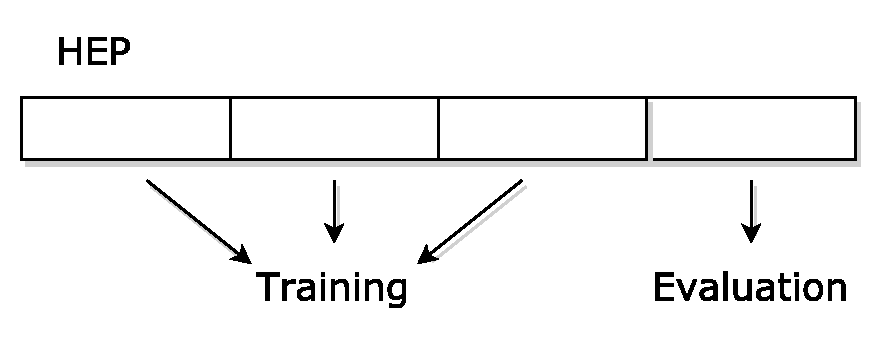
\includegraphics[width=0.36\textwidth]{Figures/CV_HEP.pdf}} & 
\subfloat[CV CORA]{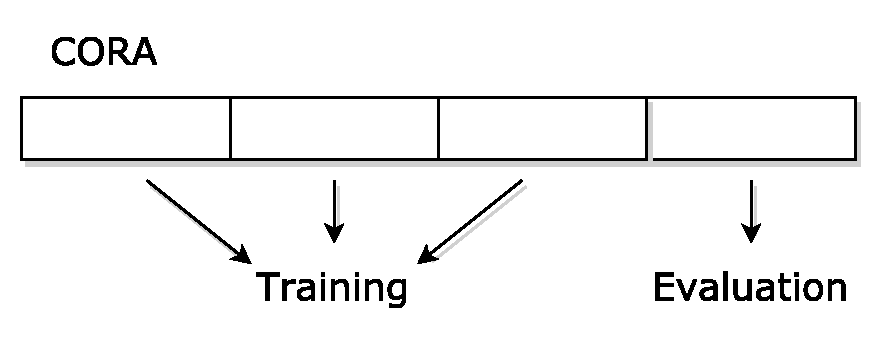
\includegraphics[width=0.36\textwidth]{Figures/CV_CORA.pdf}}\\
\subfloat[CV HEP append CORA]{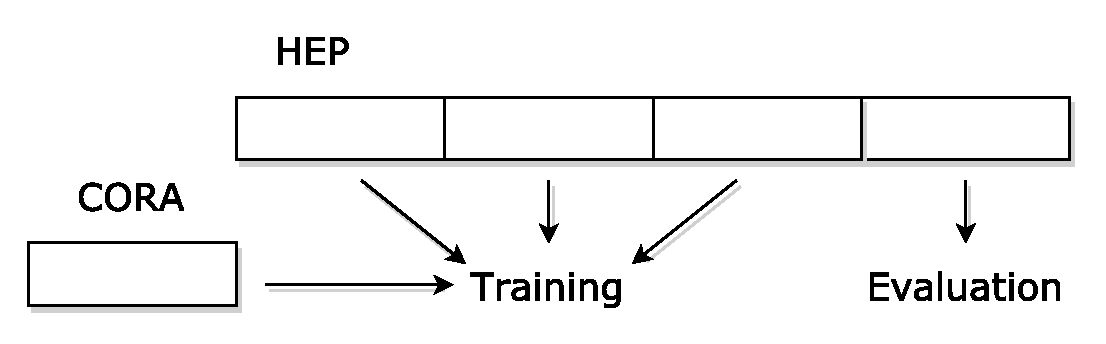
\includegraphics[width=0.45\textwidth]{Figures/CV_HEPappCORA.pdf}} & 
\subfloat[CV CORA append HEP]{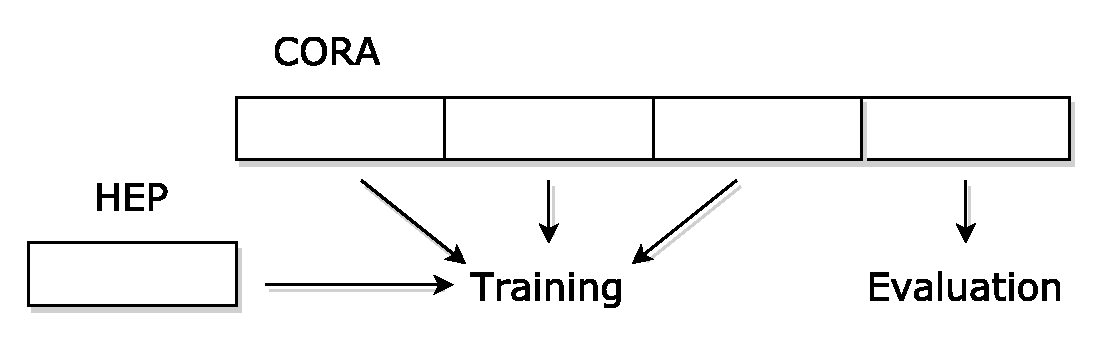
\includegraphics[width=0.45\textwidth]{Figures/CV_CORAappHEP.pdf}}\\ 
\multicolumn{2}{c}{\subfloat[CV HEP + CORA]{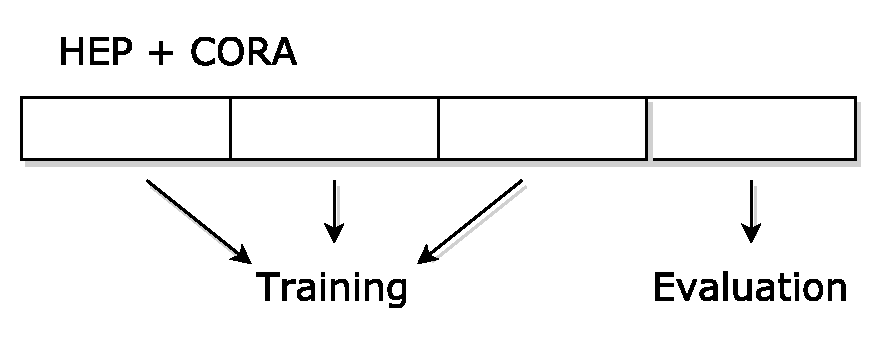
\includegraphics[width=0.36\textwidth]{Figures/CV_HEP+CORA.pdf}}} \\
\end{tabular}
\caption{The different cross-validation configurations used in our experiments. Figures (A) and (B) show cross-validation on HEP and CORA sets independently, and (E) on their combination. Figures (C) and (D) show cross-validation on the HEP and CORA datasets respectively, appending the other at training time.}
\label{fig:cv}
\end{figure}

The variety of $66$ experiments that we cross-validated are presented in Table \ref{fig:cv}, organised into 8 categories. We also distinguish by model, running some experiments for both models, and some for one alone. Generally speaking, we chose feature engineering ideas with a particular model in mind, that is, either \emph{header} or \emph{segmentation}. Finally, we distinguish by the data configurations. For dictionary-based features, which may be derived from a baseline feature file alone, we may try all data configurations. However, as we do not have access to the original PDF papers for the CORA dataset, we cannot extract our new features. In these cases, our cross-validation was performed on our own purely HEP dataset.

\begin{table}[h]
\begin{center}
\begin{tabular}{ | p{0.2\linewidth} | p{0.25\linewidth} | p{0.15\linewidth} | p{0.3\linewidth} |}
\hline
Feature Category & Variations & Models & Data\\
\hline
Baseline & - & Segmentation, header & CORA, CORA app. HEP, CORA + HEP, HEP, HEP app. CORA \\
\hline
Baseline & - & Header & HEP app. 1/3 CORA, HEP app. 2/3 CORA \\
\hline
Dictionaries & 1\textsuperscript{st} order, 2\textsuperscript{nd} order, 3\textsuperscript{rd} order & Segmentation, header & HEP, HEP app. CORA \\
\hline
Dicts. + Stops & 1\textsuperscript{st} order, 2\textsuperscript{nd} order, 3\textsuperscript{rd} order, stops only & Segmentation, header & HEP, HEP app. CORA \\
\hline
Regularisation & $\sigma^2=0$, $\sigma^2=\exp\{-6\}$, $\sigma^2=\exp\{-5\}$, $\sigma^2=\exp\{-4\}$, $\sigma^2=\exp\{-3\}$, & Header & HEP \\
\hline
Token Extension & First 5 words, first 10, first 15, first 20 & Segmentation & HEP \\
\hline
Block Size & Height, width, height \& width, area & Header & HEP \\
\hline
Levenshtein Distance & $T_1 = 0.05$, $T_1 = 0.1$, $T_1 = 0.2$, $T_1 = 0.4$, $T_1 = 0.8$, ($T_1 = 0.1, T_2 = 0.4$), All & Segmentation & HEP \\
\hline
Character Classes & Binary, decimal (round down), decimal (round), decimal (20 point) & Segmentation & HEP \\
\hline
\end{tabular}
\caption[A summary of our experiments, organised by category, models trained for, and data configurations used.]{A summary of our experiments, organised by category, models trained for, and data configurations used.}
\label{table:experiments}
\end{center}
\end{table}

\section{Comparison with \emph{refextract}}
\label{sec:refextract}

As a first result for GROBID, we compare it with \emph{refextract}, the existing solution for automatic reference extraction at CERN. \emph{refextract} is an example of a \emph{stylistic analysis} tool (see Section \ref{sec:solutionmethods}), as it employs regular expressions in a heuristic framework for metadata extraction. As previously mentioned, \emph{refextract} is incomplete and greatly lacking in both breadth and depth of detail. It is capable only of retrieving references\footnote{A comparatively easy task; GROBID's citation model usually performs at a significantly higher accuracy than, say, its \emph{header} model.}, and the classification itself is quite basic. Since the modelling of reference fields differs between the two, a comparison is difficult to make. Our results will at least be indicative, however, and we are able to make reasonable comparisons across the most important fields. The dataset for the comparison consists of 60 articles coming from the SCOAP$^3$ online repository\footnote{Scoap$^3$ (Sponsoring Open Consortium for Open Access Publishing in Particle Physics) is an open access digital library hosted at CERN, backed by an international partnership of research institutions.}.

Unlike \emph{refextract}, GROBID requires two separate models to classify the citations of a given article: the \emph{reference-segmenter} and \emph{citation} models\footnote{Strictly speaking, there is another model, (full) \emph{segmentation}, above the \emph{reference-segmenter}, and so \emph{citation} accuracy depends on this also. But because one focus of our work is to improve this model, we permit this omission.}. The \emph{reference-segmenter} model is the simplest model in GROBID's arsenal, and is responsible for segmenting a reference list block into individual references. Therefore, the accuracy of the citation model is ultimately subject to the accuracy of the reference block inputs supplied to it by the \emph{reference-segmenter} above. The results for training and evaluating the \emph{reference-segmenter} on 60 SCOAP$^3$ papers with an 80--20 split are given in Table \ref{table:referencesegmenterresults}. The results show the \emph{reference-segmenter} is extremely accurate. In fact, only 5 token misclassifications out of 622 were made for the <label> class, and from a grand total of 12,981.

\begin{table}[h]
\begin{center}
\begin{tabular}{|c|cccc|}
\hline
label           & accuracy  & precision  & recall   & f1 \\
\hline
<label>         & 99.96     & 100        & 99.2     & 99.6\\
<reference>     & 99.96     & 99.96      & 100      & 99.98\\
\hline
(micro average) & 99.96     & 99.96      & 99.96    & 99.96  \\
(macro average) & 99.96     & 99.98      & 99.6     & 99.79  \\
\hline
\end{tabular}
\caption[Token-level evaluation results for reference segmentation.]{Token-level evaluation results for reference segmentation.}
\label{table:referencesegmenterresults}
\end{center}
\end{table}

The most significant difference between the tools is the set of classes modelled. \emph{refextract} attempts only to classify to the minimum detail required for identifying the originating document within INSPIRE-HEP. Therefore, there are no equivalents to GROBID's classes, <volume>, <pages>, and so on. Rather, these parts of references are absorbed into other, higher-level classes, and are indicated by a dash (-) in the results table, Table \ref{table:citationcomparison}. Comparisons can be made, however on fields, <title>, <author>, <journal>, and <date>. There we see the superiority of GROBID over \emph{refextract}. Note that here the \emph{citation} model was not trained on the evaluation set, and in particular this may explain its dismal performance in precision for the date field, and recall for \emph{pubnum}. The dataset instances contained a recurring publication number that was almost uniformly misclassified by GROBID as a date. Notice that this is an example of a domain specificity of HEP papers. Had we trained on these papers, we could expect an improvement. That \emph{refextract} has reported perfect recall is a result of a flaw in our simplistic evaluation, where missing expected classifications were simply assigned to a \emph{null} class, and so \emph{false positives} (FP) were not counted; only \emph{false negatives}. Therefore, the true performance of \emph{refextract} is upper-bounded by the figures in Table \ref{table:citationcomparison}. The table contents are one of the outputs of GROBID's evaluation utilities. For an explanation of the performance metrics, see Section \ref{subsec:evaluationmethod}.

\begin{table}[h]
\begin{center}
\begin{tabular}{|c|cccc|cccc|}
\hline
system &  \multicolumn{4}{c|}{GROBID} & \multicolumn{4}{c|}{\emph{refextract}}\\
\hline
label & accuracy & precision & recall & f1 & acc. & prec. & rec. & f1\\
\hline
<author>    & 99.85 &   99.68   &   99.75   &   99.72   & 98.33 &   100 &   92.22   &   95.95   \\
<title> &   99.59   &   98.87   &   99.25   &   99.06   & 94.89 &   100 &   71.75   &   83.55   \\
<journal>   & 98.84 &   88.87   &   93.98   &   91.35   & 97.12 &   100 &   46.78   &   63.74   \\
<volume>&   99.95   &   99.07   &   98.15   &   98.6    & -     &   -   &   -       &   -   \\
<issue> &   99.93   &   100     &   94.63   &   97.24   & -     &   -   &   -       &   -   \\
<pages> &   99.75   &   93.51   &   99.45   &   96.39   & -     &   -   &   -       &   -   \\
<date>  &   98.39   &   57.39   &   98.31   &   72.47   & 98.88 &   100 &   37.55   &   54.6    \\
<pubnum>&   98.71   &   100     &   12.96   &   22.95   & -     &   -   &   -       &   -   \\
<note>  &   99.4    &   43.75   &   35      &   38.89   & -     &   -   &   -       &   -   \\
<publisher>&99.81   &   63.46   &   94.29   &   75.86   & -     &   -   &   -       &   -   \\
<location>& 99.81   &   86.32   &   91.11   &   88.65   & -     &   -   &   -       &   -   \\
<institution>& 99.78&   25      &   25      &   25      & -     &   -   &   -       &   -   \\
<booktitle>&    98.7&   55.56   &   41.67   &   47.62   & -     &   -   &   -       &   -   \\
<web>   &   99.64   &   51.85   &   100     &   68.29   & -     &   -   &   -       &   -   \\
<editor>    &  99.93&   100     &	46.67   &   63.64   & -     &   -   &   -       &   -   \\
<tech>  &   99.95   &   83.33   &   50      &   62.5    & -     &   -   &   -       &   -   \\
\hline
(micro average) & 99.5  &   93.63   &   94.77   &   94.19 & -    &   - &   -   &   -   \\
(macro average) & 99.5  &   77.92   &   73.76   &   71.76 & -    &   -  &   -   &   -   \\
\hline
\end{tabular}
\caption[Token-level evaluation results for citations for GROBID and \emph{refextract}.]{Token-level evaluation results for citations for GROBID and \emph{refextract}.}
\label{table:citationcomparison}
\end{center}
\end{table}

\section{Results}
\label{sec:results}

As specified earlier, we use the micro average of F1 scores of all model classes to compare model performance, only looking to specific fields when more nuanced comparisons are necessary. We hereafter state F1 micro averages unless otherwise specified.

\subsection{Baseline}
\label{subsec:baslineresults}

Given the datasets available (see Section \ref{sec:data}) we are able to experiment with the combination of HEP and CORA papers, as well as subsampling the CORA dataset to find the ideal mixture. After all, in spite of the common wisdom that increasing the amount of training data will improve generalisation and model performance, it is not clear what effects combining different ground truths will have. One may imagine that generalising over a hybrid dataset might construct a misleading model when it comes to evaluate on a pure HEP dataset, especially when the CORA \emph{header} set dwarfs our HEP one. The baseline results are given in Table \ref{table:baselineresults} and these show the micro average of F1 scores (see Section \ref{sec:evaluationmethod}) for each of the data configurations. Of most importance are the scenarios involving the HEP training set taken alone, and the HEP training set appending the CORA set, as these evaluate on HEP papers only, and are the configurations used in the other experiments. Surprisingly, for the \emph{header} model, there is a degradation of performance when the CORA set is appended. We pursue this curiosity in Table \ref{table:subsampling}, where we see mixed results for \emph{subsampling} CORA data, appending an extra randomly chosen third of the data at a time. The pure HEP set with no appending of CORA yields a model $(\mu = 90.19, \sigma = 2.63)$ second only to the case where we append $2/3$ of the CORA dataset $(\mu = 90.19, \sigma = 2.63)$. The case of appending $1/3$ CORA experienced a major outlier in the third iteration of cross-validation, where it scored an F1 micro average of as little as $78.15$, performing badly across all classes. This result notwithstanding, it seems there is some value in using a hybrid dataset yet increasing the proportion of CORA papers ultimately degrades performance. This strongly supports our hypothesis that there a qualitative difference between HEP papers and general papers, and that training a successful model demands an expansion of the HEP dataset. In further sections, we see the same effect when we train on the HEP dataset and HEP appending CORA. For a visualisation of the subsampling results, see Figure \ref{fig:subsampling_micro} in Appendix \ref{AppendixB}. It should be noted, in addition, the successful predictions of our newly introduced collaboration class for the header model (see Section \ref{sec:implementation}).

\begin{table}[t]
\begin{center}
\begin{tabular}{|c|c|c|c|c|c|}
\hline
Features & Model & Variation & Data & Mean & Std.\\
\hline
\multirow{10}{*}{Baseline} & \multirow{5}{*}{Header} & \multirow{5}{*}{-} & HEP & 90.19 & 2.63\\\cline{4-6}
& & & HEP app. CORA & 89.54 & 3.76\\\cline{4-6}
& & & CORA & 82.22 & 2.03\\\cline{4-6}
& & & CORA app. HEP & 81.8 & 2.76\\\cline{4-6}
& & & HEP \& CORA & 81.02 & 1.74\\\cline{2-6}
& \multirow{5}{*}{Segmentation} & \multirow{5}{*}{-} & HEP & 92.98 & 0.79\\\cline{4-6}
& & & HEP app. CORA & 93.58 & 1.65\\\cline{4-6}
& & & CORA & 94.02 & 2.96\\\cline{4-6}
& & & CORA app. HEP & 94.39 & 2.72\\\cline{4-6}
& & & HEP \& CORA & 92.93 & 2.94\\\cline{4-6}
\hline
\end{tabular}
\caption[Mean and standard deviation for tuning the variance of the $l_2$ variance parameter.]{Mean and standard deviation for tuning the variance of the $l_2$ variance parameter.}
\label{table:baselineresults}
\end{center}
\end{table}

\begin{table}[t]
\begin{center}
\begin{tabular}{|c|c|c|c|c|c|}
\hline
Features & Model & Variation & Data & Mean & Std.\\
\hline
\multirow{4}{*}{Baseline} & \multirow{4}{*}{Header} & \multirow{4}{*}{-} & HEP & 90.19 & 2.63\\\cline{4-6}
& & & HEP app. 1/3 CORA & 89.15 & 5.75\\\cline{4-6}
& & & \textbf{HEP app. 2/3 CORA} & 92.1 & 2.43\\\cline{4-6}
& & & HEP app. CORA & 89.54 & 3.76\\\cline{4-6}
\hline
\end{tabular}
\caption[Mean and standard deviation for tuning the variance of the $l_2$ variance parameter.]{Mean and standard deviation for tuning the variance of the $l_2$ variance parameter.}
\label{table:subsampling}
\end{center}
\end{table}

In contrast, the \emph{segmentation} model generally benefitted from combining datasets, with HEP appending CORA $(\mu = 93.58, \sigma = 1.65)$ and CORA appending HEP $(\mu = 94.39, \sigma = 2.72)$ respectively improving over HEP only $(\mu = 92.98, \sigma = 0.79)$ and CORA only $(\mu = 94.02, \sigma = 2.96)$. This seems reasonable, as the HEP set in this case is larger than the CORA one (see Section), and appending the CORA dataset can assist model performance without overwhelming the HEP characteristics as it does for the \emph{header} model. Figure \ref{fig:segmentation_baseline_confusion} gives a confusion matrix for the \emph{segmentation} model evaluated with the baseline feature on the HEP training set. The main diagonal (in dark blue) shows the majority correctness of the model. Notably, the \emph{body} class (the lines belonging to the main article sections) shows a high true positive (TP) rate (observe the contrast in the \emph{body} row), but also a high number of false positives (observe the confusion in the \emph{body} column), equivalently, the false \emph{negatives} of other classes. Thus, lower precision and higher recall. This is to be expected, as \emph{body} is the dominant class for the \emph{segmentation} model, and training error is most easily minimised with a bias to the dominant class (a similar result may be seen for the \emph{abstract} class in the \emph{header} model, a visualisation of which may be seen in \ref{fig:confusion_header} in Appendix \ref{AppendixB}.). The confusion matrix also reveals large amounts of \emph{header} matter lost to the \emph{body} class. This is of greatest concern, as the extracted data ought to supply the \emph{header} model with its inputs at prediction time. Our extension (Section \ref{subsec:extensions}) allows us to see which documents these misclassifications are most attributed to.

\begin{figure}[h]
\center
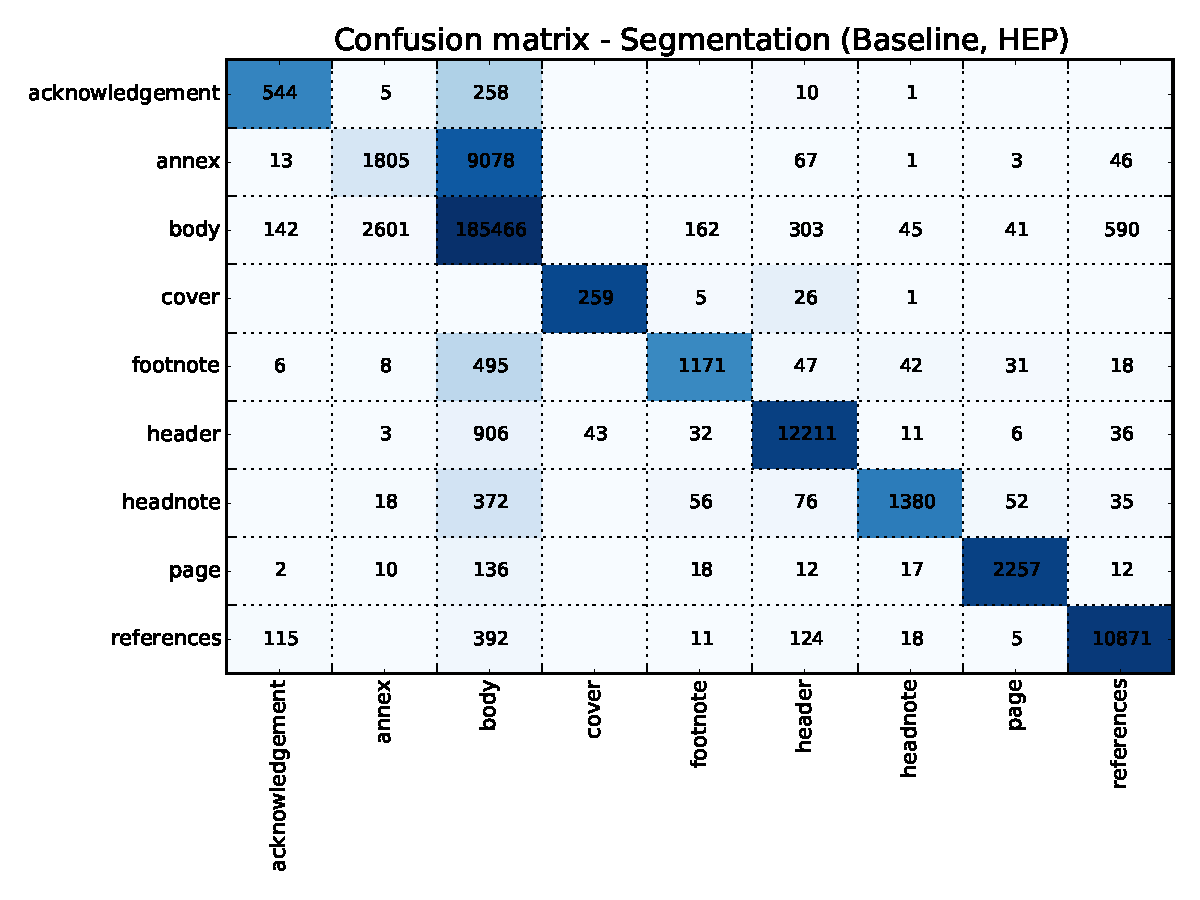
\includegraphics[width=5.5in]{Figures/baseline_confusion_segmentation.pdf}
\caption{Confusion matrix for \emph{segmentation} model with baseline features, trained on the pure HEP dataset. Counts are given, as well as a heatmap to indicate the most frequent classifications.}
\label{fig:segmentation_baseline_confusion}
\end{figure}

\subsection{Block Size}

\begin{table}[h]
\begin{center}
\begin{tabular}{|c|c|c|c|c|c|}
\hline
Features & Model & Variation & Data & Mean & Std.\\
\hline
\multirow{4}{*}{Block size} & \multirow{4}{*}{Header} & \textbf{Height} & HEP & 90.5 & 2.55\\\cline{3-6}
& & Width & HEP & 90.46 & 2.75\\\cline{3-6}
& & Height \& width & HEP  & 88.47 & 3.1\\\cline{3-6}
& & Area & HEP  & 90.42 & 2.55\\\cline{3-6}
\hline
\end{tabular}
\caption[Mean and standard deviation for subsampling CORA dataset.]{Mean and standard deviation for tuning the variance of the $l_2$ variance parameter.}
\label{table:blockshaperesults}
\end{center}
\end{table}

The results for our block size features (Table \ref{table:blockshaperesults}) were not significant, with only the most marginal differences with respect to the baseline $(\mu = 90.19, \sigma = 2.63)$. The category using both height and width features performed worst $(\mu = 88.47, \sigma = 3.1)$, showing that combining features does not necessarily improve, and may even degrade, model performance, a finding we see elsewhere also\footnote{Notably the comination of our best features for \emph{segmentation}. Future work might examine the correlation of independent features to see if a methodology for combining features may be inferred.}. The results are otherwise quite uniform. We may speculate as to the underwhelming performance of these features by noticing that block size is calculated for every token according to its membership in a contiguous group of tokens. As a result, contiguous tokens share block size identical information, and the features do nothing to \emph{characterise} the tokens in the way successful features such as \emph{dictionary} and \emph{character class} features do.

\subsection{Character Classes}

Almost every character class strategy made an improvement over the baseline (with the exception of the simple \emph{binary} variation). A visualisation of the results may be seen in Figure \ref{fig:classes_micro} in Appendix \ref{AppendixB}. Thus, the results support our intuitions about features based on character classes. The variations \emph{binary only} and \emph{decimal only} refer to the removal of the basic baseline features addressing punctuation and related line token characteristics. Interestingly, removing these \emph{improved} performance, even for the baseline case. The best result was for the \emph{20-point} variation $(\mu = 93.75, \sigma = 2.56)$ compared with the baseline, $(\mu = 92.98, \sigma = 0.79)$, corresponding to an $11\%$ reduction in error on the micro average level, as well as a $13\%$ reduction in error (F1) for \emph{references}, and a $20\%$ reduction in error for the \emph{header}, the two most important classes. The \emph{20-point} variation used a finer discretisation than the others. Future work might therefore try further refining the discretisation strategies. See Section \ref{sec:keyresults} for further comparisons.

\begin{table}[h]
\begin{center}
\begin{tabular}{|c|c|c|c|c|c|}
\hline
Features & Model & Variation & Data & Mean & Std.\\
\hline
\multirow{6}{*}{Character classes} & \multirow{6}{*}{Segmentation} & Binary & HEP & 92.82 & 1.26\\\cline{3-6}
& & Binary only & HEP & 93.5 & 2.17\\\cline{3-6}
& & Decimal (round down) & HEP & 93.57 & 2.2\\\cline{3-6}
& & Decimal only & HEP & 93.61 & 1.99\\\cline{3-6}
& & Decimal (round nearest) & HEP & 93.37 & 2.27\\\cline{3-6}
& & \textbf{Decimal (20 point)} & HEP & 93.75 & 2.56\\\cline{3-6}
\hline
\end{tabular}
\caption[Mean and standard deviation for character class discretisation strategies.]{Mean and standard deviation for character class discretisation strategies.}
\label{table:characterclassresults}
\end{center}
\end{table}

\subsection{Dictionaries}

Dictionary-based features, as described in Section \ref{subsec:dicts}, make use of domain knowledge to establish a vocabulary for \emph{header} model tokens, and give a binary indicator, modelling a token's memberships in a set of five dictionaries (titles, authors, journals, collaborations, and keywords), extracted from INSPIRE-HEP. We varied the degree of context-awareness provided to a token, creating features indicating the dictionary membership of a token's immediate neighbours, that is the tokens either side of it in the text, in addition to its own, as well as second and third degree variations. Though these features were designed with the \emph{header} model in mind, the same experimental variations were run for \emph{segmentation}. These features were expected to be more meaningful for the \emph{header} model, as they give a dimensionality reduction for a full token, mapping it to some combination of dictionaries. In the \emph{segmentation} model, this is done only for the leading word per line, and it is hard to imagine this characterising a line effectively. Predictably, the \emph{header} model benefited significantly more from these featers, with clear improvements over the baseline. When stop words were included the benefits were even greater. These results are selected for closer examination in Section \ref{subsec:keyresults}. Of further note was the near uniform superiority of the pure HEP data configuration, versus that of appending CORA data, reinforcing our findings about subsampling from the baseline results (Section \ref{subsec:baslineresults}. It is after this experiment batch that we chose to be more focused in the scenarios chosen, concentrating on the pure HEP dataset and the models expected to most benefit from the respective feature experiments.

\begin{table}[h]
\begin{center}
\begin{tabular}{|c|c|c|c|c|c|}
\hline
Features & Model & Variation & Data & Mean & Std.\\
\hline
\multirow{12}{*}{Dictionaries} & \multirow{6}{*}{Header} & \multirow{2}{*}{\textbf{1\textsuperscript{st} order}} & \textbf{HEP} & 90.75 & 2.5\\\cline{4-6}
& & & HEP app. CORA & 87.65 & 6.49\\\cline{3-6}
& & \multirow{2}{*}{2\textsuperscript{nd} order} & HEP & 90.75 & 3.01\\\cline{4-6}
& & & HEP app. CORA & 88.78 & 7.46\\\cline{3-6}
& & \multirow{2}{*}{3\textsuperscript{rd} order} & HEP & 87.67 & 7.55\\\cline{4-6}
& & & HEP app. CORA & 89.78 & 5.99\\\cline{2-6}
& \multirow{6}{*}{Segmentation} & \multirow{2}{*}{\textbf{1\textsuperscript{st} order}} & HEP & 93.56 & 1.79\\\cline{4-6}
& & & \textbf{HEP app. CORA} & 93.91 & 2.07\\\cline{3-6}
& & \multirow{2}{*}{2\textsuperscript{nd} order} & HEP & 92.16 & 1.61\\\cline{4-6}
& & & HEP app. CORA & 93.37 & 1.75\\\cline{3-6}
& & \multirow{2}{*}{3\textsuperscript{rd} order} & HEP & 93.11 & 2.6\\\cline{4-6}
& & & HEP app. CORA & 93.58 & 1.89\\
\hline
\multirow{12}{*}{Dicts. \& Stop Words} & \multirow{6}{*}{Header} & \multirow{2}{*}{1\textsuperscript{st} order} & HEP & 91.21 & 2.03\\\cline{4-6}
& & & HEP app. CORA & 88.43 & 5.92\\\cline{3-6}
& & \multirow{2}{*}{2\textsuperscript{nd} order} & HEP & 88.9 & 7.25\\\cline{4-6}
& & & HEP app. CORA & 89.87 & 5.03\\\cline{3-6}
& & \multirow{2}{*}{\textbf{3\textsuperscript{rd} order}} & \textbf{HEP} & 91.35 & 3.1\\\cline{4-6}
& & & HEP app. CORA & 89.76 & 5.99\\\cline{2-6}
& \multirow{6}{*}{Segmentation} & \multirow{2}{*}{1\textsuperscript{st} order} & HEP & 93.21 & 1.13\\\cline{4-6}
& & & HEP app. CORA & 93.48 & 2.04\\\cline{3-6}
& & \multirow{2}{*}{2\textsuperscript{nd} order} & HEP & 93.03 & 1.78\\\cline{4-6}
& & & HEP app. CORA & 93.24 & 3.49\\\cline{3-6}
& & \multirow{2}{*}{\textbf{3\textsuperscript{rd} order}} & HEP & 93.25 & 2.77\\\cline{4-6}
& & & \textbf{HEP app. CORA} & 93.58 & 2.66\\
\hline
\end{tabular}
\caption[Mean and standard deviation for tuning the variance of the $l_2$ variance parameter.]{Mean and standard deviation for tuning the variance of the $l_2$ variance parameter.}
\label{table:dictionaryresults}
\end{center}
\end{table}

\subsection{Levenshtein Distance}

All Levenshtein distance feature thresholding strategies performed better than the baseline, and the scenarios combining multiple thresholds, ($T_1 = 0.1, T_2 = 0.4$) and \emph{all}, show a clear superiority over the others. A visualisation of the results can be seen in Figure \ref{fig:levenshtein_micro} in Appendix \ref{AppendixB}. The strategy, \emph{all}, which used all of the listed thresholds to make a $5-point$ categorical variable for levenshtein distance gave the best performance, $(\mu = 94.06, \sigma = 1.81)$, compared with the baseline, $(\mu = 92.98, \sigma = 0.79)$, corresponding to a $15\%$ reduction in error on the micro average level, as well as a $20\%$ reduction in error (F1) for \emph{references}, and a $19\%$ reduction in error for the \emph{header}. These results therefore support of intuitions of the effectiveness of this feature category. Such as it is, from the laborious data acquisition process (Section \ref{sec:data}), we observed the frequency of the misclassification of delimiting token classes, \emph{page} and \emph{headnote}, as part of the \emph{body} or \emph{reference} sections, raising the FP rate for these classes, thus lowering their precision and $F_1$ scores alike. It is therefore likely that the Levenshtein distance features aided these transitional corner cases in the document segmentation.

\begin{table}[h]
\begin{center}
\begin{tabular}{|c|c|c|c|c|c|}
\hline
Features & Model & Variation & Data & Mean & Std.\\
\hline
\multirow{6}{*}{Levenshtein Distance} & \multirow{6}{*}{Segmentation} & $T_1 = 0.1$ & HEP & 93.51 & 1.37\\\cline{3-6}
& & $T_1 = 0.2$ & HEP & 92.95 & 1.19\\\cline{3-6}
& & $T_1 = 0.4$ & HEP & 93.44 & 1.28\\\cline{3-6}
& & $T_1 = 0.8$ & HEP & 93.07 & 1.07\\\cline{3-6}
& & $T_1 = 0.1, T_2 = 0.4$ & HEP & 93.78 & 1.83\\\cline{3-6}
& & \textbf{All} & HEP & 94.06 & 1.81\\\cline{3-6}
\hline
\end{tabular}
\caption[Mean and standard deviation for tuning the variance of the $l_2$ variance parameter.]{Mean and standard deviation for tuning the variance of the $l_2$ variance parameter.}
\label{table:levenshteinresults}
\end{center}
\end{table}

\subsection{Regularisation}

Our experiments in tuning the variance of the $l_2$ regularisation confirmed the earlier findings of (\cite{Peng04accurateinformation}). There is little observable difference in the performance of different choices of variance parameter, which we give in Table \ref{table:regularisationresults}. Performance is marginally worse at the extremities, namely where no penalty is imposed, and for the greatest penalty, $\sigma^2 = \exp\{-3\}$. Naturally, as a penalty is increased toward infinity, the model parameters go to 0, and performance degrades maximally. Figure \ref{fig:histogram} shows an empirical Normal distribution for a normalised model. That regularisation has little effect implies that it is difficult to overfit the model, and that the high dimensionality of the model perhaps provides in-built regularisation. Training with another algorithm supporting a different regularisation technique (such as $l_1$) could form the basis of future work.

\begin{table}[h]
\begin{center}
\begin{tabular}{|c|c|c|c|c|}
\hline
Features & Model & Variation & Mean & Std.\\
\hline
\multirow{4}{*}{Baseline} & \multirow{4}{*}{Header} & $\sigma^2 = 0$ & 90.4 & 2.58\\
& & $\mathbf \sigma^2 = \exp\{-6\}$ & 90.68 & 3.78\\
& & $\sigma^2 = \exp\{-5\}$ & 90.64 & 3.78\\
& & $\sigma^2 = \exp\{-4\}$ & 90.66 & 3.69\\
& & $\sigma^2 = \exp\{-3\}$ & 90.44 & 2.77\\
\hline
\end{tabular}
\caption[Mean and standard deviation for tuning the variance of the $l_2$ variance parameter.]{Mean and standard deviation for tuning the variance of the $l_2$ variance parameter.}
\label{table:regularisationresults}
\end{center}
\end{table}

\begin{figure}[h]
\center
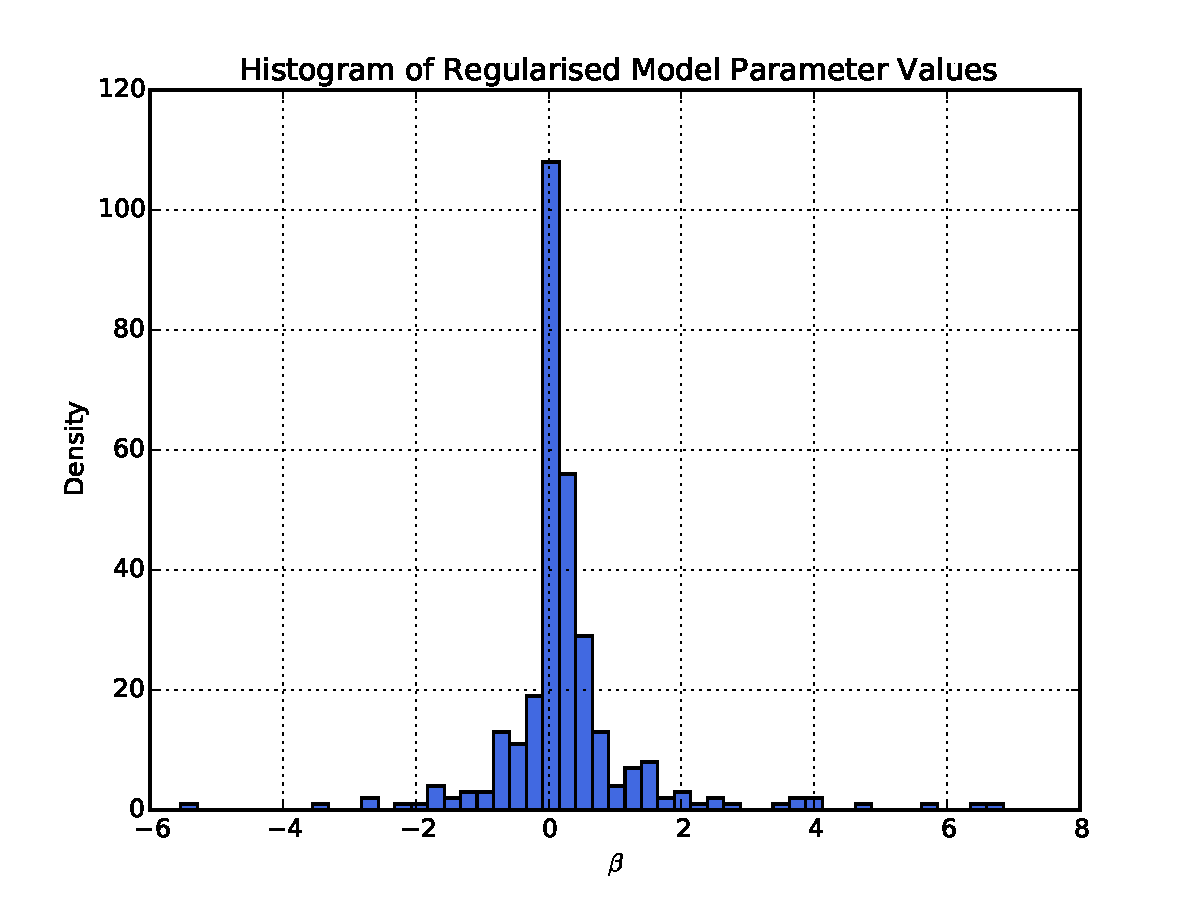
\includegraphics[width=5in]{Figures/histogram.pdf}
\caption{Distribution of model parameters with $l_2$ regularisation.}
\label{fig:histogram}
\end{figure}

\subsection{Token Extensions}
\label{subsec:tokenextensionresults}

The results for token extensions (Table \ref{table:tokenextensions}) are quite modest. None significantly exceed the baseline result with the same data configuration $(\mu = 92.98, \sigma = 0.79)$. Of note is the low variance across the variations compared with other feature categories. The result supports our earlier intuitions that though it may be helpful to establish a vocabularly that can differentiate between sections, the result of modelling each word in a line token indiviudally is a feature space that is too diffuse to learn useful indicators for lines, which are better characterised, for example, at the character- rather than word-level, such as by character class features (Section \ref{subsec:characterclasses}).

\begin{table}[h]
\begin{center}
\begin{tabular}{|c|c|c|c|c|c|}
\hline
Features & Model & Variation & Data & Mean & Std.\\
\hline
\multirow{4}{*}{Token Extension} & \multirow{4}{*}{Segmentation} & \textbf{First 5} & HEP & 93.38 & 1.6\\\cline{3-6}
& & First 10 & HEP & 92.8 & 1.08\\\cline{3-6}
& & First 15 & HEP & 93.12 & 1.5\\\cline{3-6}
& & First 20 & HEP & 93.29 & 1.75\\\cline{3-6}
\hline
\end{tabular}
\caption[Mean and standard deviation for tuning the variance of the $l_2$ variance parameter.]{Mean and standard deviation for tuning the variance of the $l_2$ variance parameter.}
\label{table:tokenextensions}
\end{center}
\end{table}

\section{Key Results}
\label{sec:keyresults}

In this section we visualise the most interesting and significant comparisons drawn from the results in Section \ref{sec:results}. We begin with the \emph{header} model, then the \emph{segmentation} model.

\subsection{Header Model}

The complexity of the \emph{header} model, modelling 17 classes (including our <collaboration> class), made finding improvements difficult. Nevertheless, the model benefitted from the five binary dictionary-based features, and further benefitted from the additional stop word feature, functioning as a $6th$ dictionary. A comparison with the baseline on the HEP dataset is visualised in Figure \ref{fig:micro_header}, showing the micro average F1 scores for each model. Dictionaries alone $(\mu = 90.75, \sigma = 2.5)$ reduced error over basline $(\mu = 90.19, \sigma = 2.63)$ by $6\%$, and dictionaries with stop words $\pm 3$ (that is, third degree contextual awareness), by $12\%$. The latter, our best result for the \emph{header} model, corresponds with a $16\%$ error reduction for <address>, $19\%$ for <author>, $54\%$ for <collaboration>, $14\%$ for <date>, and $25\%$ for <keywords>, unchanged performance for <abstract>, <affiliation>, and <title>, and a slight degradation of $8\%$ for <pubnum>.

\begin{figure}[h]
\center
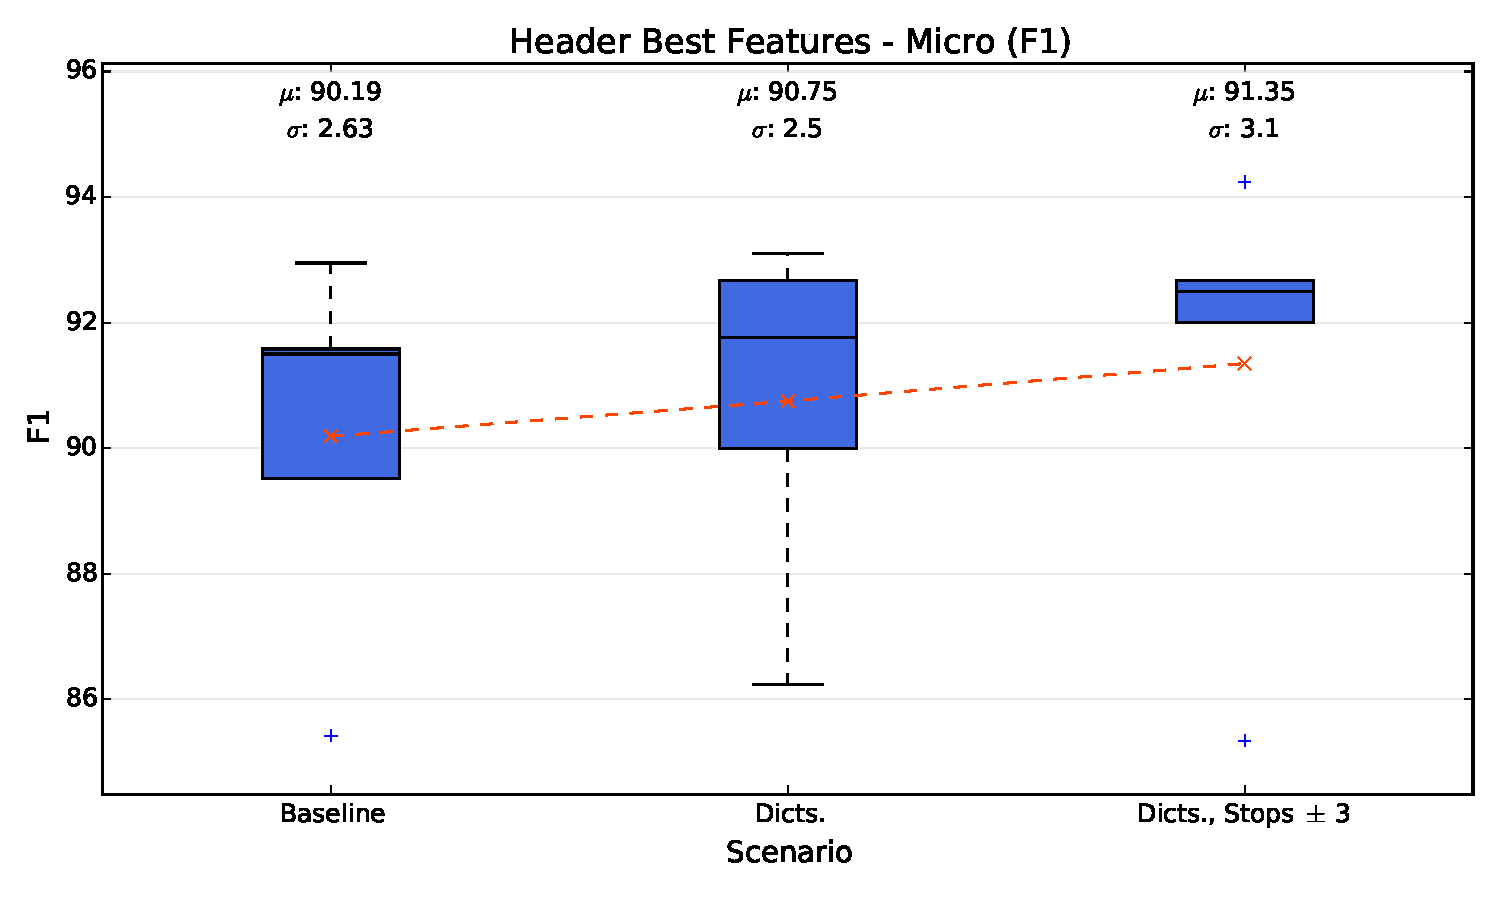
\includegraphics[width=5.5in]{Figures/micro_header.pdf}
\caption{Comparison of baseline, levenshtein and character class features on header matter.}
\label{fig:micro_header}
\end{figure}

\subsection{Segmentation Model}

\begin{figure}[b]
\center
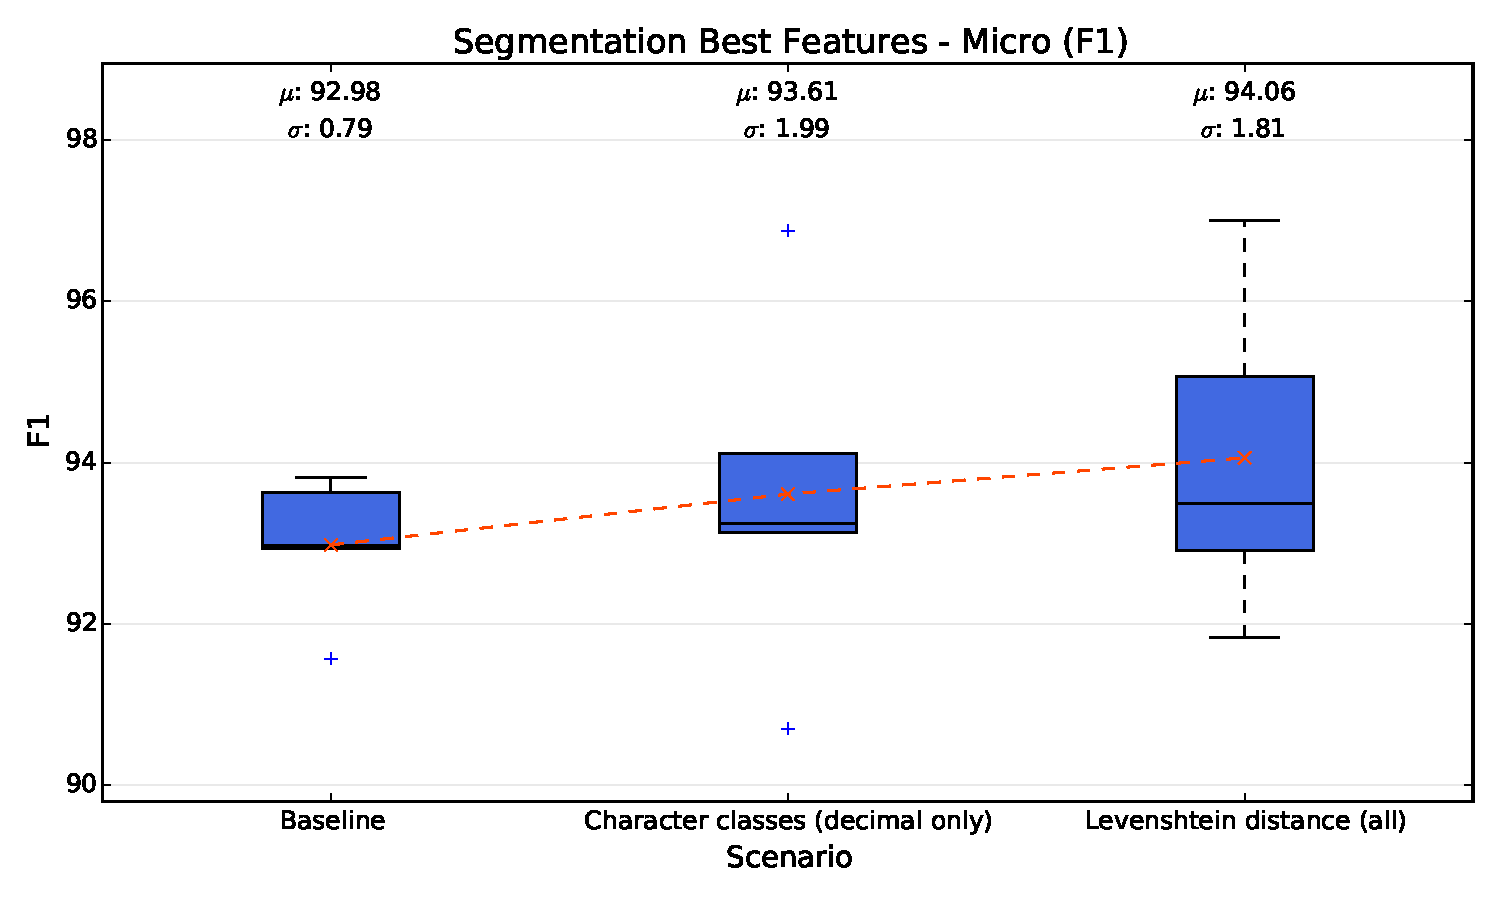
\includegraphics[width=5.5in]{Figures/micro_segmentation.pdf}
\caption{Comparison of baseline, levenshtein and character class features on header matter.}
\label{fig:micro_segmentation}
\end{figure}

For the \emph{segmentation} model, two feature categories offered significant improvements over the baseline. These categories were those of character classes (CC) and Levenshtein distance and (LD), and their best variations were respectively the decimal discretisation with related baseline features removed, and the Levenshtein distance using all thresholds to create a quinternary categorical variable. Figure \ref{fig:micro_segmentation} shows a boxplot comparing the micro average of F1 scores of these two variations with the baseline, evaluated on the pure HEP dataset. The CC variation gives an overall error reduction of $9\%$, and the LD, $15\%$. However, when we look at the most important fields, <header> and <references>, we see that though again, both models outperform the baseline, now CC leads with a $24\%$ error reduction for the <header> class, with $19\%$ for LD, and a $21\%$ error reduction for <references> versus $20\%$ for LD. The character class model is therefore excelling in the cases it was explicitly designed to improve.


\begin{figure}[h]
\center
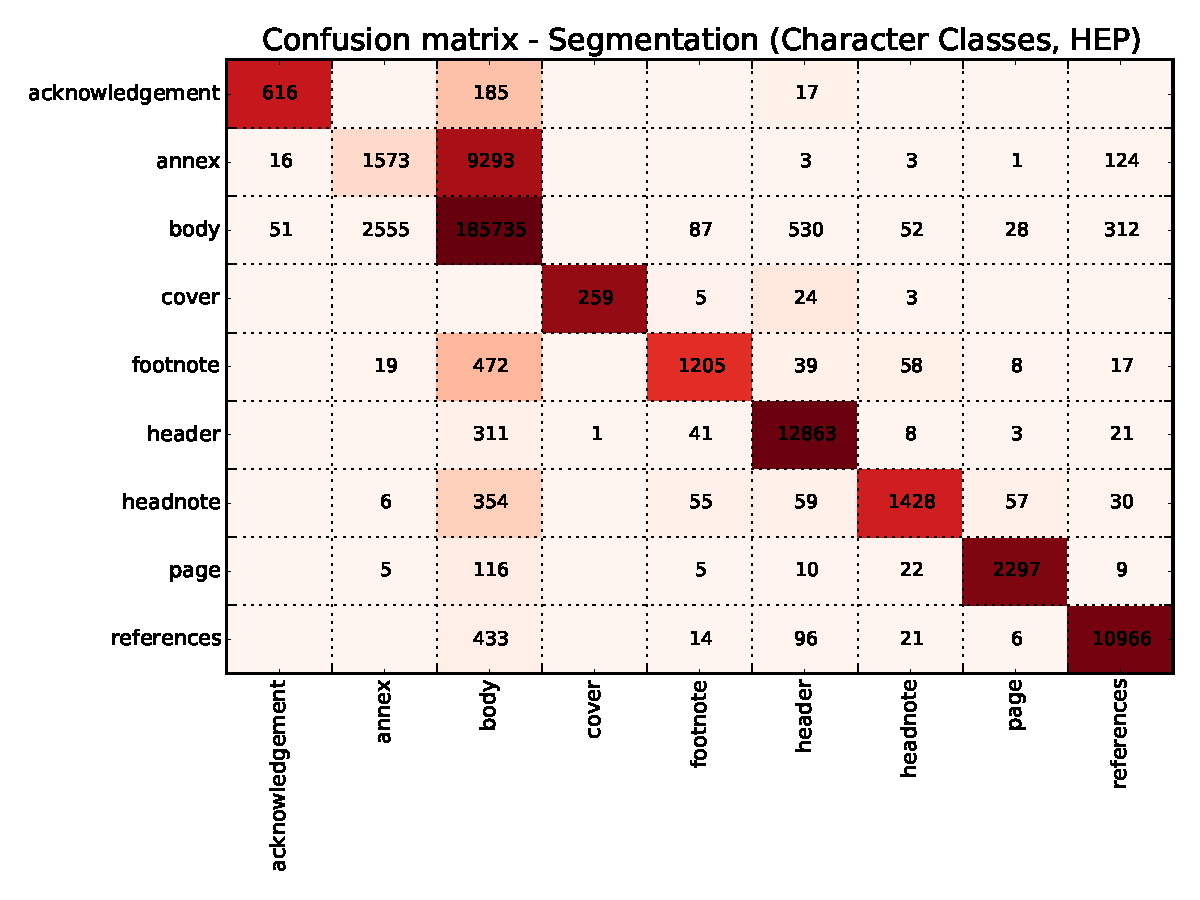
\includegraphics[width=5.5in]{Figures/classes_confusion_segmentation.pdf}
\caption{Comparison of baseline, levenshtein and character class features on header matter.}
\label{fig:confusion_segmentation}
\end{figure}

\begin{figure}[h]
\center
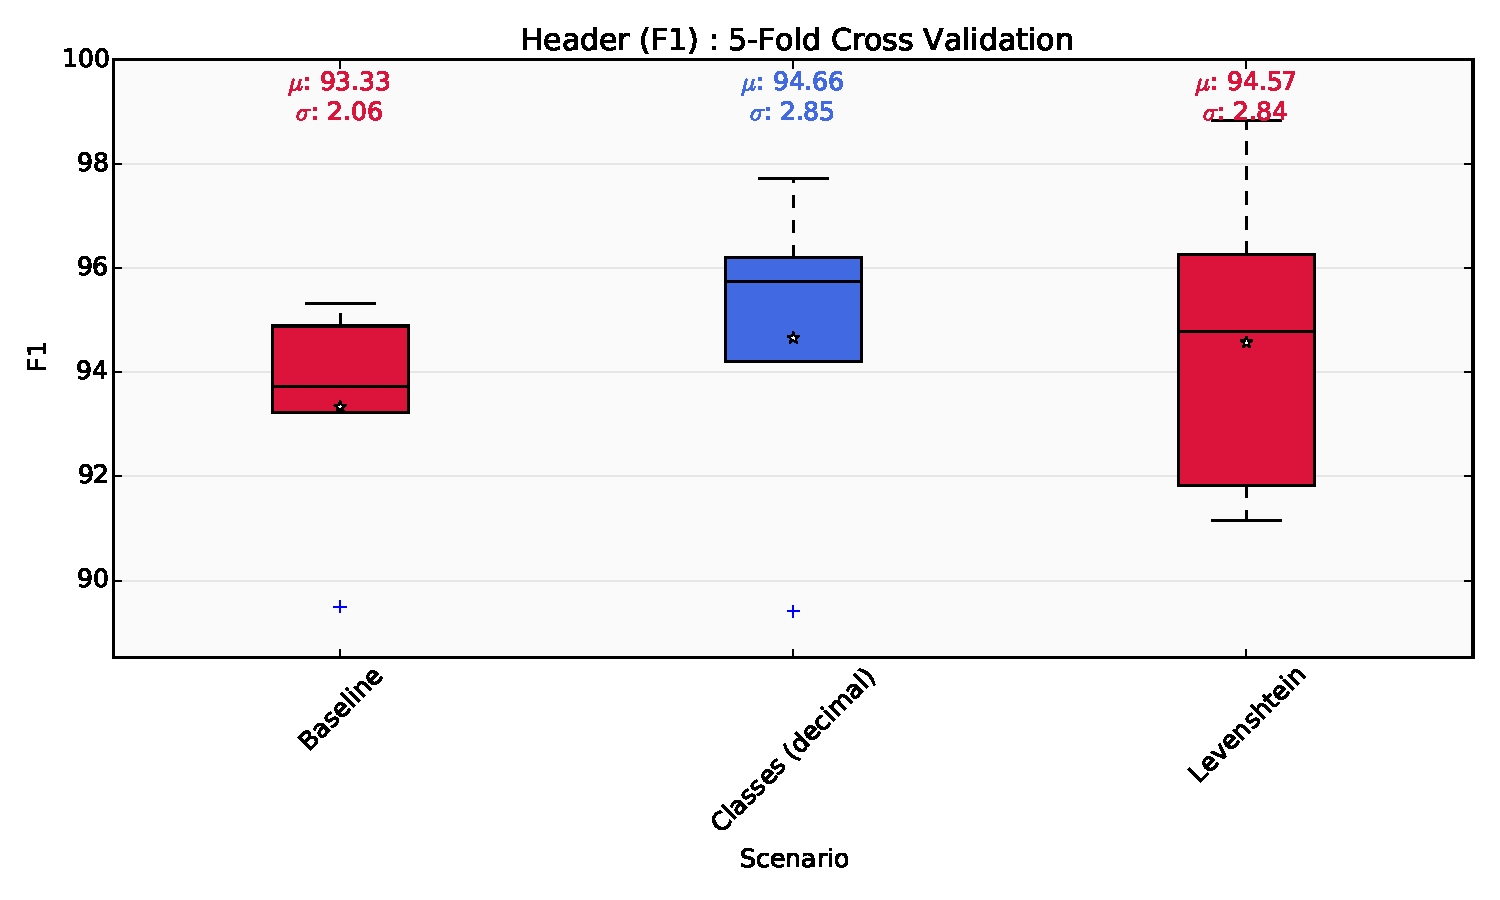
\includegraphics[width=5.5in]{Figures/header.pdf}
\caption{Comparison of baseline, levenshtein and character class features on header matter.}
\label{fig:header}
\end{figure}

\begin{figure}[h]
\center
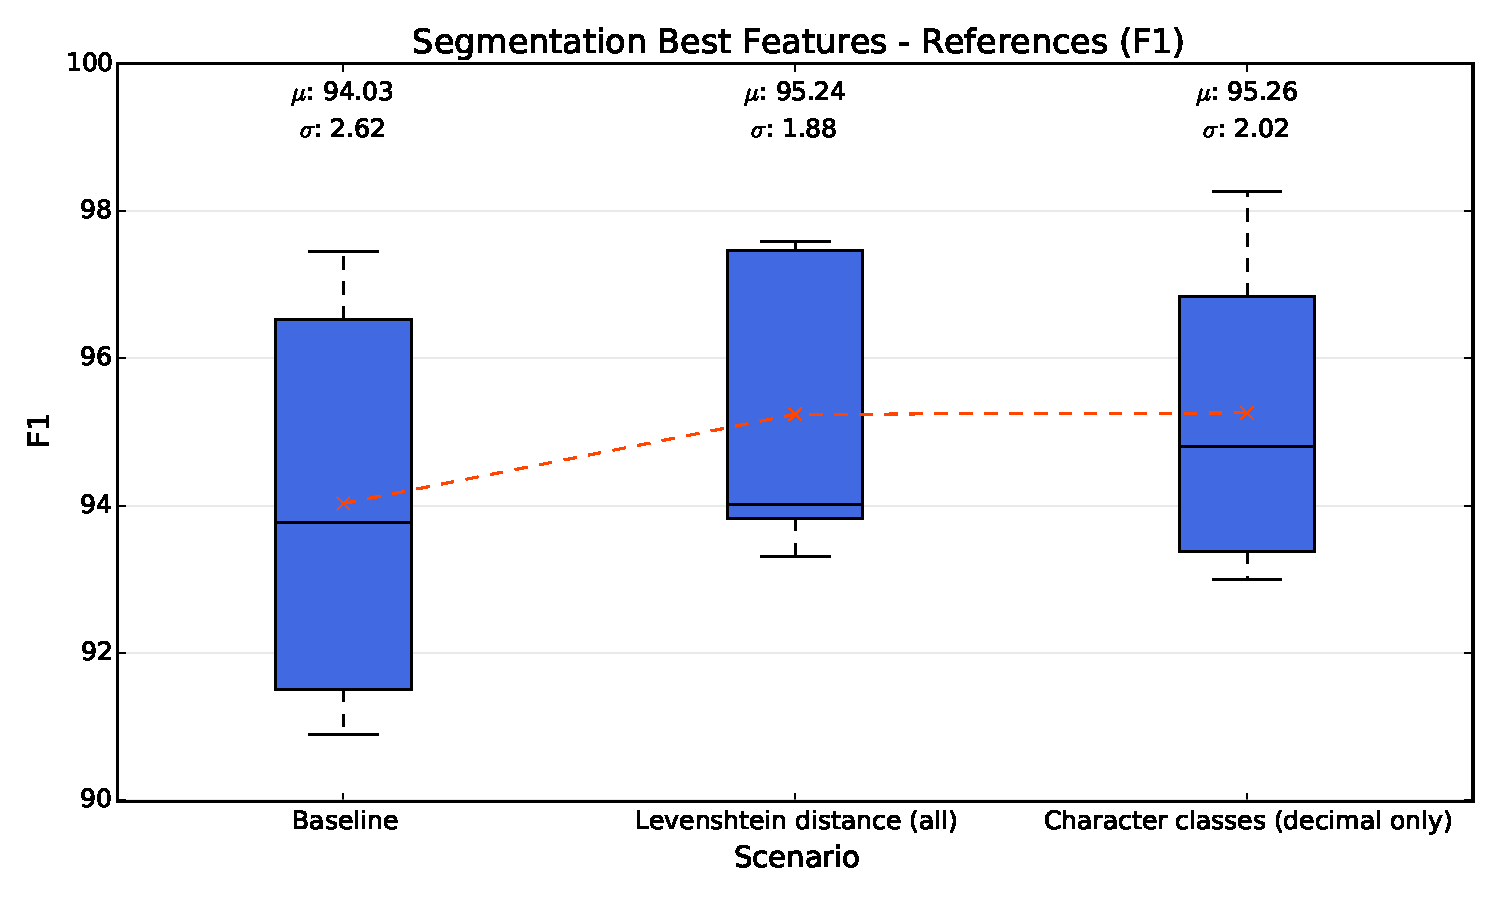
\includegraphics[width=5.5in]{Figures/references.pdf}
\caption{Comparison of baseline, levenshtein and character class features on header matter.}
\label{fig:references}
\end{figure}

The confusion matrix for character classes (decimal only) on HEP papers in Figure \ref{fig:confusion_segmentation} shows a dramatic improvement over the baseline (Figure \ref{fig:confusion_segmentation}. Of particular interest are the incease across the main diagonal, that is true positives (TP) in every class but one, <annex>.

Though the overall performance was lower, we advocate the character class features due to its magnificent performance in key fields, <header> and <references>.


